% !TeX program = xelatex
% Compile twice with XeLaTeX, or once with tectonic.
\documentclass[UTF8,a4paper,11pt,fontset=fandol]{ctexart}
\usepackage[margin=1.8cm,top=2cm,bottom=2cm]{geometry}
\usepackage{amsmath,booktabs,longtable,array,tabularx,xcolor,listings}
\usepackage{caption}
\usepackage{graphicx,float}
\usepackage[unicode,colorlinks=true,linkcolor=blue!55!black,urlcolor=blue!55!black]{hyperref}
\usepackage{xurl}
\hypersetup{pdftitle={Lab 0 实验报告：使用 OpenROAD 自动完成芯片设计},pdfauthor={}}
\setlength{\parindent}{2em}
\setlength{\parskip}{0.25em}
\setlength{\tabcolsep}{4pt}
\renewcommand{\arraystretch}{1.2}
\setlength{\emergencystretch}{2em}
\newcolumntype{P}[1]{>{\raggedright\arraybackslash}p{#1}}
\newcolumntype{R}[1]{>{\raggedleft\arraybackslash}p{#1}}
\newcommand{\code}[1]{\texttt{\detokenize{#1}}}
\newcommand{\missing}{---}
\newcommand{\derived}[1]{#1\textsuperscript{\(\dagger\)}}
\newcommand{\inherited}{0\textsuperscript{*}}
\newcommand{\groupbar}[2]{\midrule\multicolumn{#1}{l}{\bfseries #2}\\\midrule}
\captionsetup{font=small,labelfont=bf}
\lstdefinestyle{script}{language=Python,basicstyle=\ttfamily\footnotesize,
  keywordstyle=\color{blue!60!black},commentstyle=\color{green!35!black},
  stringstyle=\color{red!45!black},numbers=left,numberstyle=\tiny\color{gray},
  numbersep=6pt,breaklines=true,breakatwhitespace=false,
  columns=fullflexible,keepspaces=true,showstringspaces=false,
  frame=single,rulecolor=\color{gray!40},xleftmargin=1.7em,
  aboveskip=0.8em,belowskip=0.8em,tabsize=4}

\title{Lab 0 实验报告\\\large 使用 OpenROAD 自动完成芯片设计}
\author{Tongbin Zhao}
\date{2026.9.15}

\begin{document}
\pagestyle{plain}
\maketitle
\vspace{-2.5em}

本报告回答实验指导书 Questions 中的问题 1--5。实验对象为 ORFS 内置的
\code{designs/sky130hd/jpeg}，顶层模块为 \code{jpeg_encoder}，基线时钟周期为 \(5.0\,\mathrm{ns}\)（\(200\,\mathrm{MHz}\)）。
日志记录的 OpenROAD 版本为 \code{26Q3-2056-g41a28926b9}，
标准单元库为 \code{sky130_fd_sc_hd__tt_025C_1v80.lib}，即 TT、
\(25\,^{\circ}\mathrm{C}\)、\(1.80\,\mathrm{V}\) 条件。

下文文件路径均相对于 \code{OpenROAD-flow-scripts/flow/}。
记 \(L=\)\path{logs/sky130hd/jpeg/base/}，
\(R=\)\path{reports/sky130hd/jpeg/base/}，
\(D=\)\path{results/sky130hd/jpeg/base/}；扫描结果目录记为
\(S=\)\path{tmp/clk_period_sweep_sky130hd_jpeg_jmed41fq/}。
数值以这些目录中的已有文件为依据。

\section{问题 1：OpenROAD运行的各个阶段}

按 \(L\) 中实际存在的 21 个 \code{.log} 文件归类，OpenROAD流程包括综合、布图规划、布局、
时钟树综合、布线和收尾六个主阶段。表中的次阶段名即日志文件名去掉
\code{.log} 后的名称。两个 LEC 日志是所属主流程内部调用的等价性检查。

\small
\begin{longtable}{@{}P{1.6cm}P{5.6cm}P{9.3cm}@{}}
\caption{按日志命名划分的流程及各次阶段作用}\label{tab:stages}\\
\toprule 主阶段 & 次阶段（日志名） & 主要作用 \\\midrule
\endfirsthead
\multicolumn{3}{l}{表 \thetable\ （续）}\\
\toprule 主阶段 & 次阶段（日志名） & 主要作用 \\\midrule
\endhead
\bottomrule\endfoot
1 综合 & \code{1_1_yosys_canonicalize} & 读取 RTL、展开参数化模块并整理设计层次，生成供后续综合使用的 RTLIL 中间表示。\\
& \code{1_2_yosys} & 将行为级设计转换、优化并映射到 sky130hd 标准单元，输出门级网表和约束。\\
& \code{1_synth} & 在 OpenROAD 中载入综合网表、工艺库和约束，生成综合后的 ODB 数据库并统计设计规模。\\
\midrule
2 布图规划 & \code{2_1_floorplan} & 建立 die、core、标准单元行与布线轨道，调整 tie 单元及缓冲器，并生成初始时序报告。\\
& \code{2_2_floorplan_macro} & 为宏单元安排位置；本设计没有宏单元，日志明确记录跳过宏布局。\\
& \code{2_3_floorplan_tapcell} & 插入 10,174 个 tapcell，为阱和衬底提供连接。\\
& \code{2_4_floorplan_pdn} & 生成芯片电源分配网络 PDN，建立标准单元区域的供电结构。\\
\midrule
3 布局 & \code{3_1_place_gp_skip_io} & 在暂不考虑 I/O 引脚位置的条件下执行初步全局布局。\\
& \code{3_2_place_iop} & 根据初步布局优化边界 I/O 引脚位置，以改善引脚到内部单元的连线。\\
& \code{3_3_place_gp} & 执行时序和可布线性驱动的全局布局，并插入端口缓冲器及进行设计修复。\\
& \code{3_4_place_resized} & 基于布局估计寄生参数，检查并修复单元驱动能力和电气设计约束。\\
& \code{3_5_place_dp} & 将单元合法化到具体 site 和行，优化镜像方向，并检查布局合法性和时序。\\
\midrule
4 时钟树综合 & \code{4_1_cts} & 为 4,384 个时钟接收端构建时钟树，并在真实时钟延迟下修复 setup/hold 时序。\\
& \code{4_rsz_lec_check} & 检查 CTS 后时序修复前后的逻辑等价性，本次结果为 \code{Circuits are IDENTICAL}。\\
\midrule
5 布线 & \code{5_1_grt} & 执行全局布线、生成布线引导，并进行寄生估计、时序修复与天线修复。\\
& \code{5_2_route} & 完成精确轨道和过孔上的详细布线，迭代消除布线规则违例，并继续修复天线问题。\\
& \code{5_3_fillcell} & 在标准单元间隙放置 60,829 个 filler，补齐单元行的物理连续性。\\
\midrule
6 收尾 & \code{6_1_fill} & 执行金属填充阶段入口；本次实际操作为复制布线数据库，日志没有金属填充插入记录。\\
& \code{6_report} & 完成最终电源连接、网表与 DEF 输出、RC 提取、STA、IR drop 分析和结果图像生成。\\
& \code{6_final_lec_check} & 比较综合后的逻辑网表与最终逻辑网表，本次等价性检查通过。\\
& \code{6_1_merge} & 用 KLayout 将最终 DEF 与单元版图合并为 GDS，检查单元版图匹配及孤立单元。\\
\end{longtable}
\normalsize

收尾阶段按实际依赖关系列出：\code{6_final_lec_check} 在 \code{6_report}
内部执行，\code{6_1_merge} 使用最终 DEF 生成版图。
本次 \code{6_1_merge.log} 报告所有 LEF 单元都有匹配的 GDS/OAS 单元，且最终版图没有 orphan cell；
最终产物为 \(D\) 下的 \code{6_final.gds}。

\section{问题 2：设计规模、时序和 DRC}

本题中的实力数量统计数据来源于\path{OpenROAD-flow-scripts/flow/reports/sky130hd/jpeg/base/synth_stat.txt} （以下简称\path{stat.txt}）。、
“总实例”包含逻辑单元和实际插入的物理单元，在\path{stat.txt}中对应cell一栏数据；
“时序实例”指寄存器/触发器，在\path{stat.txt}中对应 \code{sky130_fd_sc_hd__edfxtp_*}和\code{sky130_fd_sc_hd__dfrtp_*}这两类数据的\code{count}之和；
“组合实例”包含其余所有标准单元项目，即逻辑门、反相器、缓冲器和常量单元。综合统计列出 \(4,318+64+2=4,384\) 个时序单元。
表中上标 \(\dagger\) 表示依据相邻已知网表/统计及该次阶段的单元增删记录推算或沿用，
并非该阶段独立输出的分类统计。无独立时序报告的次阶段标记为“\missing”。

表中WNS/TNS 均为 setup 指标，单位为 ns；优先采用同名 JSON 中的
\code{timing__setup__ws} 和 \code{timing__setup__tns}。
由于按照\path{lab0_guide.pdf}要求用默认的时钟周期$5ns$跑完整的flow，时序优化的最终结果依然无法满足\code{setup}时序约束，
因此本表中已记录的 worst setup slack 全为负数。

DRC 列专指\textbf{详细布线规则违例数}，未计入布局合法性、天线违例、
max slew/max capacitance 检查或工具 \code{errors__count} ，数据来源为 \path{OpenROAD-flow-scripts/flow/logs/sky130hd/jpeg/base/5_2_route.json}。
\path{OpenROAD-flow-scripts/flow/reports/sky130hd/jpeg/base/5_route_drc.rpt}为空，因此可以判定最后drc为例数目为$0$。

\begingroup\fontsize{8.5}{11}\selectfont
\begin{longtable}{@{}P{4.8cm}R{1.45cm}R{1.25cm}R{1.5cm}R{1.85cm}R{1.9cm}R{1.25cm}@{}}
\caption{各主、次阶段的设计规模与质量指标（基线 \(T=5.0\) ns）}\label{tab:metrics}\\
\toprule 次阶段 & 总实例 & 时序实例 & 组合实例 & WNS/ns & TNS/ns & DRC \\\midrule
\endfirsthead
\multicolumn{7}{l}{表 \thetable\ （续）}\\
\toprule 次阶段 & 总实例 & 时序实例 & 组合实例 & WNS/ns & TNS/ns & DRC \\\midrule
\endhead
\bottomrule\endfoot
\multicolumn{7}{l}{\bfseries 1 综合}\\\midrule
\code{1_1_yosys_canonicalize} & \missing & \missing & \missing & \missing & \missing & \missing\\
\code{1_2_yosys} & 31,722 & 4,384 & 27,338 & \missing & \missing & \missing\\
\code{1_synth} & 31,722 & \derived{4,384} & \derived{27,338} & \missing & \missing & \missing\\
\groupbar{7}{2 布图规划}
\code{2_1_floorplan} & 30,811 & \derived{4,384} & \derived{26,427} & -49.6288 & -58,959.2 & \missing\\
\code{2_2_floorplan_macro} & \derived{30,811} & \derived{4,384} & \derived{26,427} & \missing & \missing & \missing\\
\code{2_3_floorplan_tapcell} & \derived{40,985} & \derived{4,384} & \derived{26,427} & \missing & \missing & \missing\\
\code{2_4_floorplan_pdn} & \derived{40,985} & \derived{4,384} & \derived{26,427} & \missing & \missing & \missing\\
\groupbar{7}{3 布局}
\code{3_1_place_gp_skip_io} & \derived{40,985} & \derived{4,384} & \derived{26,427} & \missing & \missing & \missing\\
\code{3_2_place_iop} & \derived{40,985} & \derived{4,384} & \derived{26,427} & \missing & \missing & \missing\\
\code{3_3_place_gp} & 45,041 & \derived{4,384} & \derived{30,483} & -0.871954 & -149.194 & \missing\\
\code{3_4_place_resized} & 45,041 & \derived{4,384} & \derived{30,483} & -0.871954 & -149.194 & \missing\\
\code{3_5_place_dp} & 45,041 & \derived{4,384} & \derived{30,483} & -0.844211 & -152.148 & \missing\\
\groupbar{7}{4 时钟树综合}
\code{4_1_cts} & 46,045 & 4,384 & \derived{31,487} & -0.663021 & -124.882 & \missing\\
\code{4_rsz_lec_check} & \missing & \missing & \missing & \missing & \missing & \missing\\
\groupbar{7}{5 布线}
\code{5_1_grt} & 46,155 & \derived{4,384} & \derived{31,554} & -0.780836 & -166.273 & \missing\\
\code{5_2_route} & \derived{46,210} & \derived{4,384} & \derived{31,554} & \missing & \missing & 0\\
\code{5_3_fillcell} & \derived{107,039} & \derived{4,384} & \derived{31,554} & \missing & \missing & \inherited\\
\groupbar{7}{6 收尾}
\code{6_1_fill} & \derived{107,039} & \derived{4,384} & \derived{31,554} & \missing & \missing & \inherited\\
\code{6_report} & 107,039 & 4,384 & 31,554 & -0.610091 & -87.6604 & \inherited\\
\code{6_final_lec_check} & \missing & \missing & \missing & \missing & \missing & \missing\\
\code{6_1_merge} & \derived{107,039} & \derived{4,384} & \derived{31,554} & \missing & \missing & \inherited\\
\end{longtable}
\endgroup

布线 DRC 的数据来自 \code{5_2_route.json} 的
\code{detailedroute__route__drc_errors}=0。上标 * 表示沿用这一检查结果，
因为 filler、收尾或 GDS 合并阶段没有重新执行 DRC。
现有文件没有独立 signoff DRC 结果。

\section{问题 3：时钟周期扫描与最大频率}\label{sec:q3}

\subsection{实验脚本}

本实验通过脚本 \path{scripts/sta_clock_period_sweep.py} 进行。
\textbf{\hyperref[app:script]{点击跳转到报告末尾的完整实验脚本（附录~\ref*{app:script}）}}。
脚本以已经完成布线的基线为输入，流程如下：
\begin{enumerate}
  \item 从 \(D\) 读取 \code{6_final.odb}（最终物理设计及连接）、
  \code{6_final.sdc}（基线时钟和 I/O 等约束）与
  \code{6_final.spef}（已提取的布线寄生参数）。
  通过原设计 \code{config.mk} 和 \code{load.tcl} 载入相同的工艺/时序库；
  从 \(L\) 的 \code{5_2_route.json} 读取并保存基线 DRC 数。
  \item 对每个扫描周期产生独立的 \code{scan.sdc}，同步修改
  \code{clk} 和虚拟时钟 \code{vclk_clk} 的 \code{create_clock -period}。
  两者基线周期均为 5 ns。输入/输出延迟仍保持 1 ns，
  虚拟时钟延迟仍保持 1.175 ns，其余约束不变。
  脚本将 ns 转换为秒，再通过 \code{sta::time_sta_ui} 转成库的原生时间单位。
  \item 在 \code{tmp} 中为每个周期建立独立目录，链接已有 ODB/SPEF，
  用 \code{make run} 执行临时生成的 \code{sta.tcl}。
  Tcl 调用 \code{load_design 6_final.odb scan.sdc}，
  设置 propagated clock 并读取已有 SPEF，随后在 OpenROAD 内重跑 OpenSTA。
  因此重分析对象是\textbf{布线完成后的最终设计状态}，对应收尾阶段的最终 STA；
  此过程不执行综合、布局、CTS、布线或重新提取寄生。
  \item 输出 worst setup slack、WNS、TNS，以及各路径组至多 5 条 setup/hold 路径；
  解析 \code{sta.log}，生成 \code{summary.csv} 和 \code{summary.txt}。
  setup 是否通过由未经低精度取整的 worst setup slack 是否非负判定。
\end{enumerate}

脚本保留 generated-clock 关系；对显式 waveform 或基线周期不一致的主/虚拟时钟会拒绝扫描，
以免在未经核对时改变时钟语义。它虽输出 hold 路径报告，但汇总中的
\code{setup_pass} 只表示本题要求的 setup 判据。

\(S\) 的 \code{experiment.json} 记录了本次实验的时钟频率范围为 5.60--5.70 ns、步长 0.01 ns，共 11 点。
这与脚本默认步长 0.1 ns 不同；与记录一致的运行命令为：
\begin{lstlisting}[basicstyle=\ttfamily\small,breaklines=true,frame=single]
cd OpenROAD-flow-scripts/flow
python3 scripts/sta_clock_period_sweep.py \
  --platform sky130hd --design jpeg --min 5.6 --max 5.7 --step 0.01
\end{lstlisting}

\subsection{扫描结果}

表 \ref{tab:sweep} 的基线来自 \code{6_report.json}，11 个扫描点来自
\(S\) 的 \code{summary.csv}，并与各周期的 \code{sta.log} 核对。
正的 worst setup slack 与 WNS 不同：OpenSTA 的 \code{report_wns} 在没有负 slack 时返回 0。
因此同时列出两者，避免把通过时的裕量误写为 WNS。

\begin{table}[htbp]
\centering\small
\caption{固定最终布线设计的时钟周期扫描}\label{tab:sweep}
\begin{tabular}{@{}rrrrrrc@{}}
\toprule
\(T\)/ns & \(f\)/MHz & 最差 setup slack/ns & WNS/ns & TNS/ns & DRC & setup\\\midrule
5.00（基线） & 200.000000 & -0.610091 & -0.610091 & -87.6604 & 0 & 失败\\
5.60 & 178.571429 & -0.010091039 & -0.010091039 & -0.010091039 & 0 & 失败\\
5.61 & 178.253119 & -0.000091038 & -0.000091038 & -0.000091038 & 0 & 失败\\
5.62 & 177.935943 & 0.009908963 & 0.000000000 & 0.000000000 & 0 & 通过\\
5.63 & 177.619893 & 0.019908965 & 0.000000000 & 0.000000000 & 0 & 通过\\
5.64 & 177.304965 & 0.029908964 & 0.000000000 & 0.000000000 & 0 & 通过\\
5.65 & 176.991150 & 0.039908968 & 0.000000000 & 0.000000000 & 0 & 通过\\
5.66 & 176.678445 & 0.049908966 & 0.000000000 & 0.000000000 & 0 & 通过\\
5.67 & 176.366843 & 0.059908967 & 0.000000000 & 0.000000000 & 0 & 通过\\
5.68 & 176.056338 & 0.069908969 & 0.000000000 & 0.000000000 & 0 & 通过\\
5.69 & 175.746924 & 0.079908967 & 0.000000000 & 0.000000000 & 0 & 通过\\
5.70 & 175.438596 & 0.089908972 & 0.000000000 & 0.000000000 & 0 & 通过\\
\bottomrule
\end{tabular}
\end{table}

基线的 setup 裕量为负，由题目给出的关系，可先估计限制周期
\[
T_{\min,\mathrm{est}}=T-s_{\mathrm{worst}}
=5.0-(-0.610091)\approx5.610091\ \mathrm{ns}.
\]
其中 \(s_{\mathrm{worst}}\) 使用带符号的 worst setup slack。
扫描在 5.61 ns 时仍有 \(-0.000091038\) ns（约 \(-0.091038\) ps）的负裕量，
即使低精度报告可能显示为 \(-0.00\)，仍应判为失败。
5.62 ns 时裕量为 \(+0.009908963\) ns，WNS 和 TNS 都为 0。

因此，\textbf{本次扫描中最小的通过周期为 5.62 ns，对应最大已验证频率}
\[
\boxed{f_{\max,\mathrm{tested}}=\frac{1000}{5.62}
=177.935943\ \mathrm{MHz},\qquad N_{\mathrm{DRC}}=0.}
\]
0.01 ns 的扫描步长只能把 setup 边界夹在 \((5.61,5.62]\) ns 内，不能证明精确最小周期恰为 5.62 ns。
由各点 \(T-s_{\mathrm{worst}}\) 得到的边界估计约为 5.610091 ns，
对应约 178.250227 MHz；这也是最终低精度 \code{period_min=5.61}、
\code{fmax=178.25} 报告的来源，\textbf{属于估计值，未在该精确周期上实测通过}。
各点 DRC 都为 0，是因为固定版图并沿用同一次详细布线检查结果，而不是逐点重新执行 DRC。

\section{问题 4：运行时间占比与瓶颈}

在基线 21 个日志中，19 个有 \code{Elapsed time}，可以直接提取墙钟时间。
两个 LEC 日志没有独立的 \code{Elapsed time}，但它们由
\code{4_1_cts} 和 \code{6_report} 内部同步调用，耗时已包含在相应父阶段中，故不重复累加。
其日志首末时间戳分别相差约 2.749 s 和 7.042 s，仅用于交叉核对。
采用每个主阶段所含非重复次阶段的墙钟时间之和 \(t_i\)，计算
\[
\mathrm{share}_i=\frac{t_i}{\sum_j t_j}\times100\%,\qquad
\sum_jt_j=1654.24\ \mathrm{s}=27\ \mathrm{min}\ 34.24\ \mathrm{s}.
\]

\begin{table}[htbp]
\centering
\caption{六个主阶段的运行时间及占比}\label{tab:runtime-main}
\begin{tabular}{@{}lrr@{}}
\toprule 主阶段 & 墙钟时间/s & 占比/\%\\\midrule
1 综合 & 36.45 & 2.20\\
2 布图规划 & 4.82 & 0.29\\
3 布局 & 76.48 & 4.62\\
4 时钟树综合 & 63.24 & 3.82\\
5 布线 & 1440.26 & 87.06\\
6 收尾 & 32.99 & 1.99\\\midrule
总计 & 1654.24 & 100.00\\\bottomrule
\end{tabular}
\end{table}

\small
\begin{longtable}{@{}P{2cm}P{7.5cm}rr@{}}
\caption{次阶段耗时明细；占比的分母仍为整个基线流程的 1654.24 s}\label{tab:runtime-sub}\\
\toprule 主阶段 & 次阶段 & 时间/s & 占比/\%\\\midrule
\endfirsthead
\multicolumn{4}{l}{表 \thetable\ （续）}\\
\toprule 主阶段 & 次阶段 & 时间/s & 占比/\%\\\midrule
\endhead
\bottomrule\endfoot
1 综合 & \code{1_1_yosys_canonicalize} & 1.88 & 0.11\\
 & \code{1_2_yosys} & 33.57 & 2.03\\
 & \code{1_synth} & 1.00 & 0.06\\
2 布图规划 & \code{2_1_floorplan} & 3.10 & 0.19\\
 & \code{2_2_floorplan_macro} & 0.39 & 0.02\\
 & \code{2_3_floorplan_tapcell} & 0.40 & 0.02\\
 & \code{2_4_floorplan_pdn} & 0.93 & 0.06\\
3 布局 & \code{3_1_place_gp_skip_io} & 3.96 & 0.24\\
 & \code{3_2_place_iop} & 0.41 & 0.02\\
 & \code{3_3_place_gp} & 47.03 & 2.84\\
 & \code{3_4_place_resized} & 8.61 & 0.52\\
 & \code{3_5_place_dp} & 16.47 & 1.00\\
4 时钟树综合 & \code{4_1_cts} & 63.24 & 3.82\\
 & \code{4_rsz_lec_check} & \multicolumn{2}{l}{已包含于父阶段，不另计}\\
5 布线 & \code{5_1_grt} & 252.87 & 15.29\\
 & \code{5_2_route} & 1186.35 & 71.72\\
 & \code{5_3_fillcell} & 1.04 & 0.06\\
6 收尾 & \code{6_1_fill} & 0.59 & 0.04\\
 & \code{6_report} & 29.30 & 1.77\\
 & \code{6_final_lec_check} & \multicolumn{2}{l}{已包含于父阶段，不另计}\\
 & \code{6_1_merge} & 3.10 & 0.19\\
\end{longtable}
\normalsize

\textbf{耗时的主要瓶颈是详细布线。}单独的 \code{5_2_route} 用时 1186.35 s，
约占总耗时的 71.72\%；连同全局布线，布线主阶段占 87.06\%。
详细布线需要为大量引脚寻找可达接入点，并在具体轨道和过孔上反复搜索、检查规则和修复冲突，因此程序运行耗时
较长。

\section{问题 5：ERROR、WARNING/WARN 及 waive 判断}

按照题干，对 \(L\) 下全部 21 个 \code{.log} 和 \(S\) 下 22 个
\code{sta.log}/\code{make.log} 进行不区分大小写的
\code{ERROR}、\code{WARNING}、\code{WARN} 检索；\(R\) 下两个天线检查日志也已检索，未发现这些等级的消息。
\textbf{没有发现 ERROR 级别报错}；基线共 127 条警告消息，扫描日志中 22 条均为
\code{STA-0450}，其中 \code{make.log} 和 \code{sta.log} 是同一次运行的重复记录。
不能为了填表而将 WARNING 改写为 ERROR。下表保留实际级别，并将同原因的重复消息合并。
waive 指是否可在本实验目的下接受该消息，不等于证明设计通过完整签核。

\small
\begin{longtable}{@{}P{4.3cm}P{6.5cm}P{5.7cm}@{}}
\caption{实际日志中的报错/警告原因与处置判断}\label{tab:warnings}\\
\toprule 主阶段 / 次阶段 & 原始消息与原因 & 是否可 waive\\\midrule
\endfirsthead
\multicolumn{3}{l}{表 \thetable\ （续）}\\
\toprule 主阶段 / 次阶段 & 原始消息与原因 & 是否可 waive\\\midrule
\endhead
\bottomrule\endfoot
全流程与扫描 STA & 未检出 \code{ERROR} & -- \\
\midrule
1 综合 /\newline\code{1_1_yosys_canonicalize} & \code{Warning: Replacing memory ... with list of registers}，共 4 条：\code{sresult}、\code{q_pipe}、\code{s_pipe}、\code{d_pipe} 以寄存器形式展开；见第 32、36--38 行。 & 可以。该实现使用标准单元寄存器，综合检查为 0 problems；应接受其面积代价，不能将这些数组当成已映射的 SRAM。\\
\midrule
1 综合 /\newline\code{1_1_yosys_canonicalize} & \code{Warning: Ignoring module ... because it contains processes (run 'proc' command first)}，共 74 条；第 117--190 行发生在早期 \code{OPT_CLEAN}，此时模块仍含行为过程。 & 可以在本次流程中接受。跳过的是该次清理，后续 \code{1_2_yosys} 执行过程转换和映射；最终综合统计 processes 为 0，\code{synth_check.txt} 报告 0 problems。\\
\midrule
1 综合 / \code{1_synth}；\newline
4 CTS / \code{4_1_cts}；\newline
6 收尾 / \code{6_report} & \code{Warning: master sky130_ef_sc_hd__decap_12 has signal pins but no liberty cell}，共 5 条；对应第 17 行、110/457 行、14/15 行，LEF 中的 decap master 没有匹配的 Liberty 单元。 & 本次可以。\code{2_1_floorplan.log} 明确说明该 master 已载入但未使用；最终实例也未使用它，故不形成待分析的逻辑时序弧。\\
\midrule
2 布图规划 /\newline\code{2_1_floorplan} & \code{WARNING IFP-0028}（第 18 行）：core 左下角从 \((1.000,1.000)\) 对齐到 \((1.380,2.720)\)\,\(\mu\mathrm{m}\)，以适配 site/row 网格。 & 可以。属于合法的网格对齐，后续应以实际 core 坐标和面积为准。\\
\midrule
2 布图规划 /\newline\code{2_4_floorplan_pdn} & \code{WARNING PDN-1051}（第 10--11 行）：\code{CORE_macro_grid_1/2} 没有对应实例。 & 可以。本设计宏单元数为 0，\code{2_2_floorplan_macro} 已记录无宏；标准单元电网仍正常生成。\\
\midrule
3 布局 /\newline\code{3_3_place_gp} & \code{WARNING GRT-0281}（第 157 行）：\code{Net clk has a large fanout of 4385 terminals}，CTS 之前时钟尚直接连接大量触发器。 & 可以作为 CTS 前的阶段性警告接受。后续 CTS 对 4,384 个 sink 建树；不能把 CTS 前的原始扇出当成最终时钟网的扇出。\\
\midrule
4 CTS / \code{4_1_cts}；\newline
5 布线 / \code{5_1_grt} & \code{WARNING RSZ-0062: Unable to repair all setup violations}（第 452、589 行）；修复后仍存在 setup 违例。 & \textbf{不能作为 5 ns 时序通过而 waive。}最终 WNS 仍为负；只能将基线作为未收敛结果如实保留，并在问题 3 中另行报告放宽周期后的 setup 通过结果。\\
\midrule
5 布线 / \code{5_1_grt}、\code{5_2_route} & \code{WARNING DRT-0349: LEF58_ENCLOSURE with no CUTCLASS is not supported}，各 10 条；分别见第 12--21、13--22 行，工具跳过 \code{mcon}、\code{via} 至 \code{via4} 的有关规则。 & \textbf{不能据此宣称完整 DRC 通过。}若用于制造签核，须用支持这些规则的 DRC 检查补证，现有结果不足以无条件 waive。\\
\midrule
5 布线 / \code{5_1_grt}、\code{5_2_route}、\code{5_3_fillcell}；\newline
6 收尾 / \code{6_report}；\newline
扫描 / 各 \code{period_*/sta.log} & \code{WARNING STA-0450: virtual clock vclk_clk can not be propagated}；基线 4 条，扫描每点 1 条（另有 make 日志副本）；\code{set_propagated_clock [all_clocks]} 同时选中了虚拟时钟。 & 可以。虚拟时钟没有实际时钟树，本应保持理想时钟；真实 \code{clk} 仍按传播时钟分析，虚拟时钟的 I/O 约束仍保留。\\
\midrule
5 布线 /\newline\code{5_1_grt} & \code{WARNING RSZ-0104: Net ... only has one pin}，第 170--196 行共 12 个单引脚网络；可能为悬空或未使用连接，需核对设计意图。 & 后续 LEC 通过提供逻辑等价性的支持，在认可jpeg这个设计没有问题的情况下可以waive，更严谨的做法是检查jpeg设计中的端口连接是否符合设计意图。\\
\midrule
5 布线 /\newline\code{5_1_grt} & \code{WARNING FLW-0010: more than one clock found. Skipping sdc update}（第 686 行）；脚本发现 \code{clk} 和 \code{vclk_clk}，跳过只支持单时钟的参考 SDC 更新。 & 本次可以。原有两时钟约束被保留，\code{6_final.sdc} 中两者均为 5 ns；问题 3 的脚本又同步修改了两者。不能理解为自动更新已经执行。\\
\midrule
6 收尾 /\newline\code{6_report} & \code{WARNING GUI-0076}（第 69 行）：\code{XDG_RUNTIME_DIR} 未设置，Qt 使用 \code{/tmp/runtime-} 作为默认目录。 & 可以。属于 GUI 运行目录提示，结果图像和最终产物已生成，不是设计时序或物理违例。\\
\end{longtable}
\normalsize



\section{问题 6：版图与关键路径}
完成$5ns$时钟周期的完整flow运行后，在\path{OpenROAD-flow-scripts/flow}目录下运行
\begin{lstlisting}[basicstyle=\ttfamily\small,frame=single]
make gui_final
\end{lstlisting}
即可打开OpenROAD的GUI界面，根据用户导引中的相关指南打开\path{Heat map-Routing Congestion}图层，显示
结果如下：
\begin{figure}[H]
    \centering
    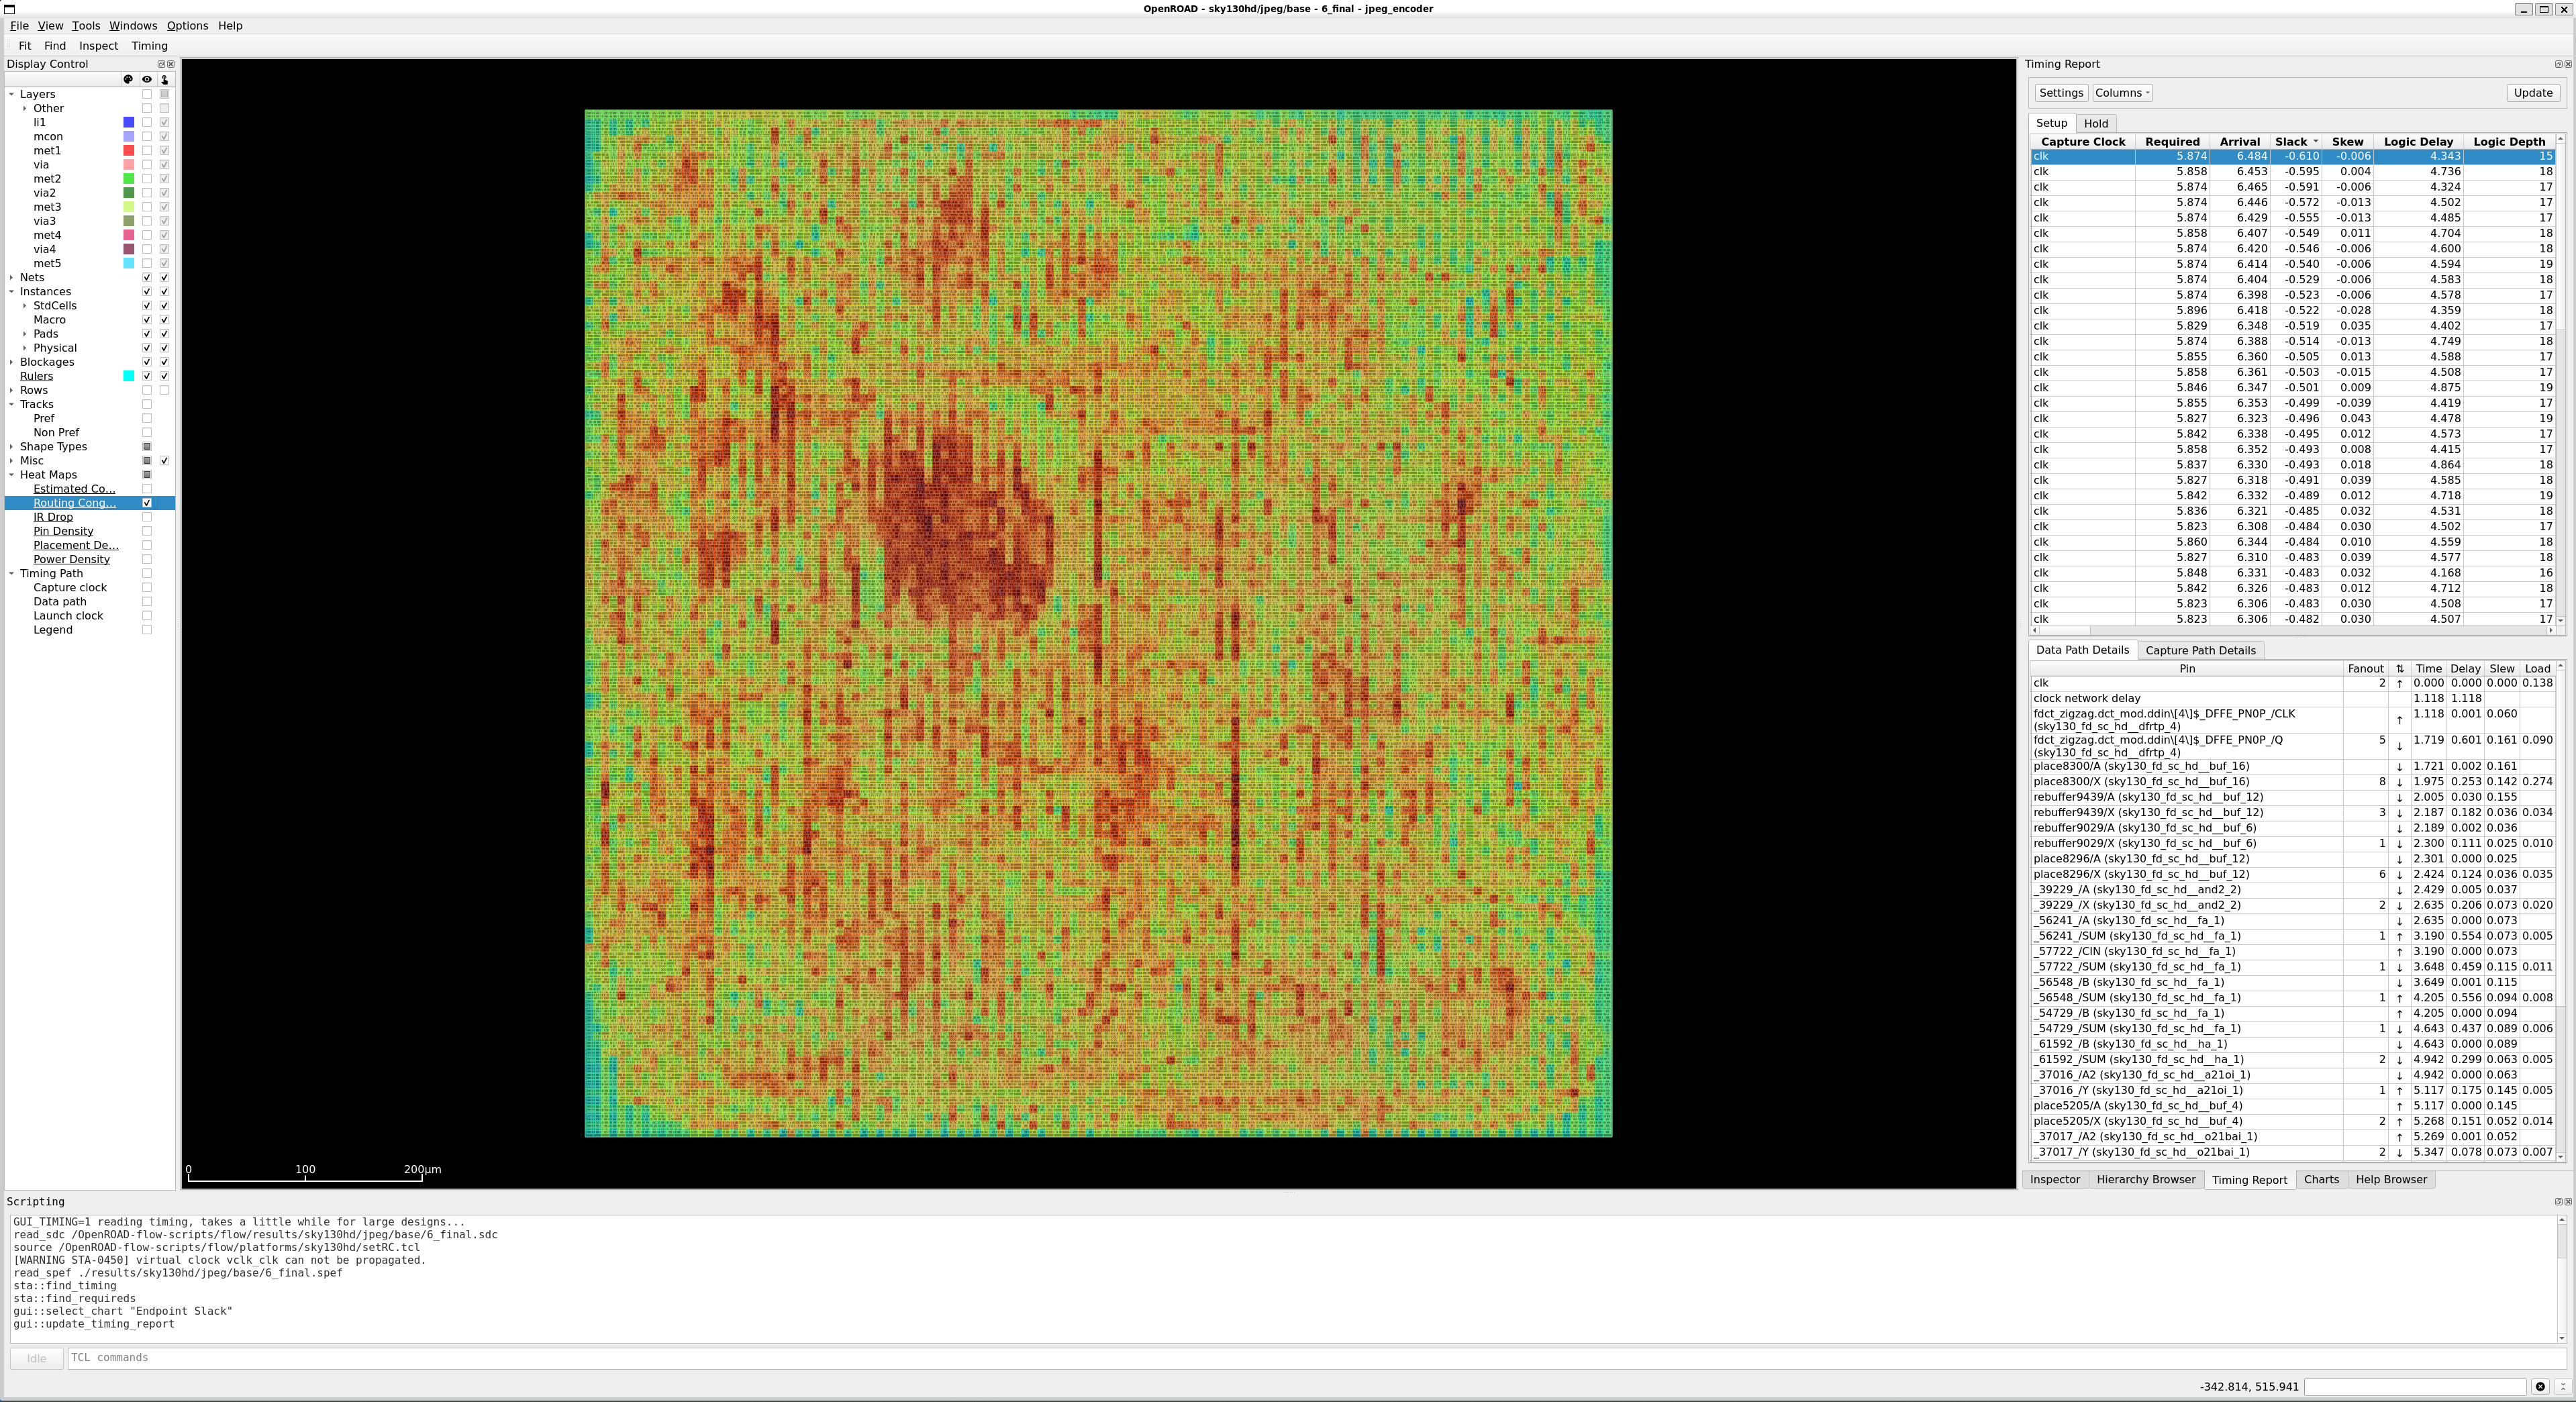
\includegraphics[width=\linewidth]{assets/route_congestion.png}
    \caption{5 ns 基线最终版图的布线拥塞热力图}
    \label{fig:route-congestion}
\end{figure}

在右侧的\code{Timing Report}菜单栏中点击选中\code{WNS}数值最小的一项，此条即本设计中的关键路径，可在GUI中
显示出来。为了关键路径清晰可见此处关掉了 Layers 图层。
\begin{figure}[H]
    \centering
    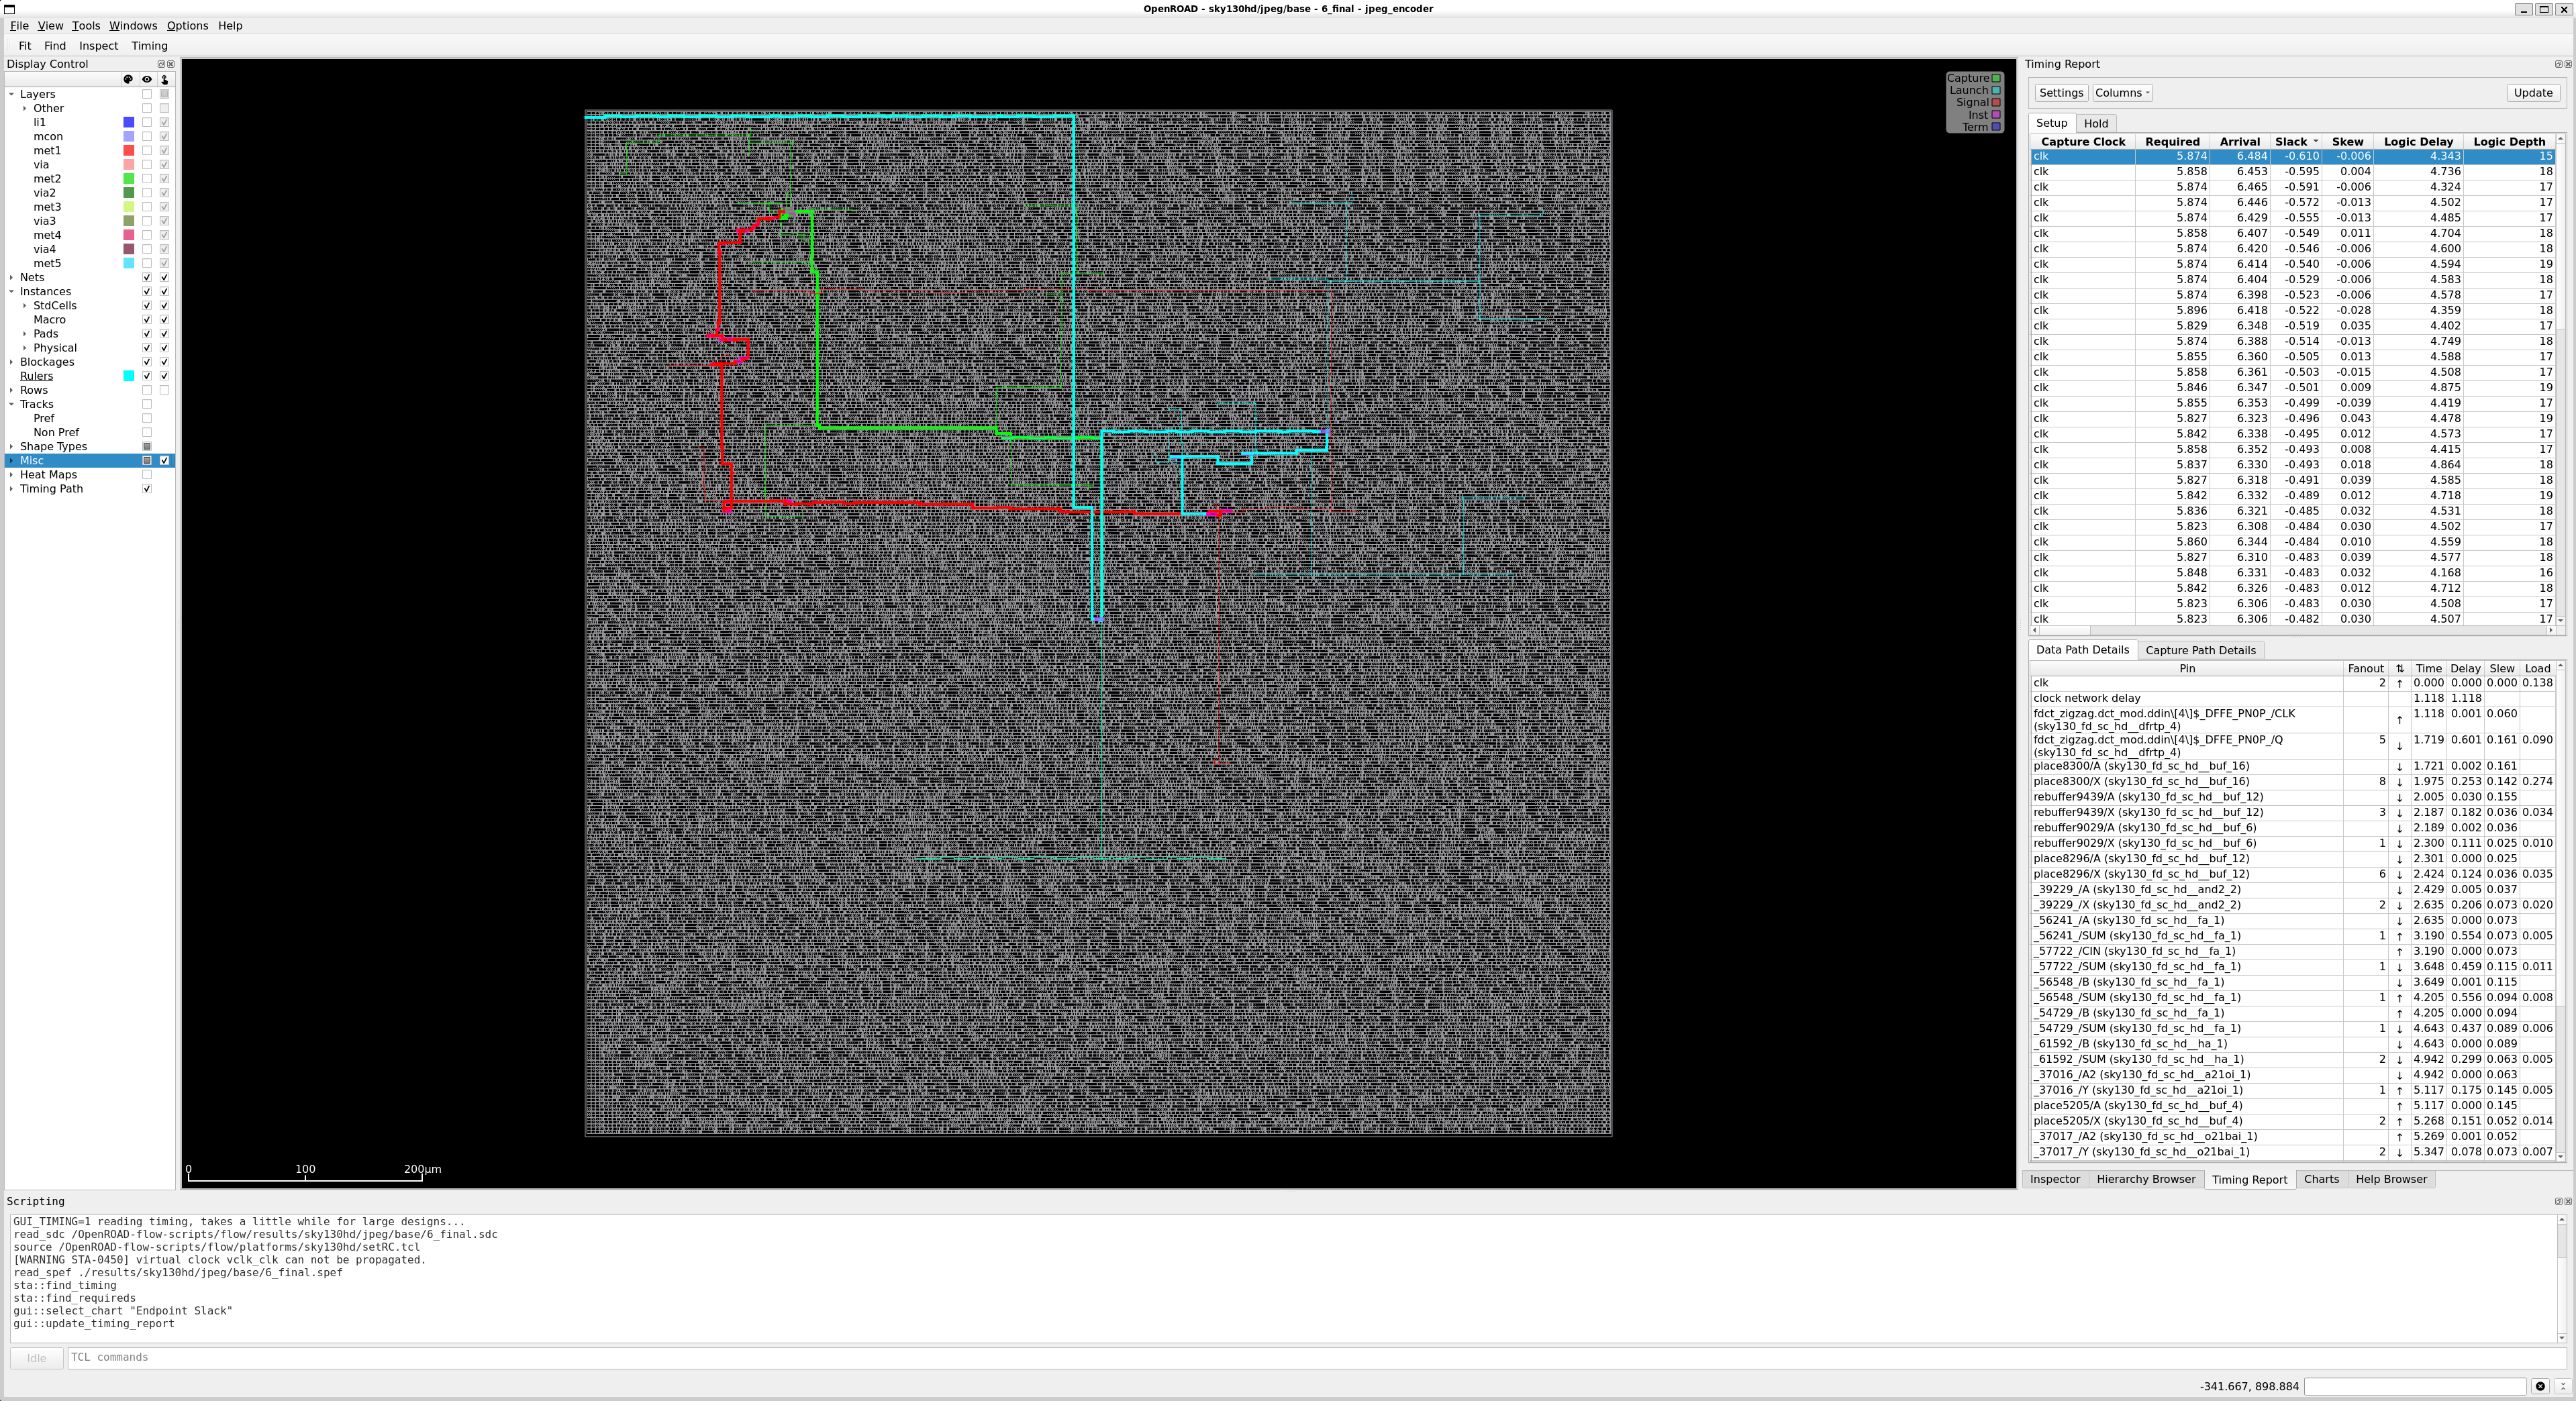
\includegraphics[width=\linewidth]{assets/critical_path.png}
    \caption{5 ns 基线最终版图的关键时序路径}
    \label{fig:critical-path}
\end{figure}


\clearpage
\appendix

\section{AI使用记录}
本次lab0完成过程中，作者主要在\code{OpenSTA}重跑扫描时钟频率、基于OpenROAD输出结果的统计工作、报告撰写和实验环境配置过程中的\code{debug}四个方面使用了AI工具，其中后两项主要
工程性的工作，不属于\code{lab0}的核心内容，因此此处不作详细展示。前两项中使用的\code{Prompt}分别如下：
\subsection{OpenSTA 重跑扫描时钟频率}
\begin{enumerate}
    \item 如何只重跑opensta？
    \item AutoTuner运行扫惨的时候会重跑整个flow吗？还是如果只有SDC\_CLOCK\_PERIOD参数的话它就是只跑最后的OpenSTA的？
    \item 请帮我完善一下前面的这个脚本，具体包含下面的步骤：

    \begin{enumerate}
        \item 规定clk\_period扫描实验的所有输出放在./tmp目录下，我会在容器里面的/OpenROAD-flow-scripts/flow执行实验启动的命令
        \item 扫描的参数为clk\_period，扫描范围从5.6到5.7 ns，间隔为0.1ns
        \item 目前我已经跑完了sky130hd平台下的jpeg完整的后端flow，输出在report, log, results, objects这四个文件夹里面，你可以根据需要读取他们
        \item 最终给我一个完整的实验脚本并告诉我运行的方式。实验脚本直接放在scripts目录下，启动方式在对话里面写给我
    \end{enumerate}
    \item 帮我修改一下这个脚本，让它能够接受如下输入字段：

    \begin{enumerate}
        \item platform，为需要跑clk\_period扫描的设计使用的platform
        \item design，为需要跑clk\_period扫描的设计的nick name
        \item min，为clk\_period扫描的最小值，单位是ns
        \item max，为clk\_period扫描的最大值，单位是ns
        \item step，为clk\_period扫描的步长，单位是ns
        \item work\_home，为输出的根目录，按照当前代码的默认值就是 tmp 这个文件夹
    \end{enumerate}
\end{enumerate}

\subsection{基于 OpenROAD 输出结果的统计工作}
\begin{enumerate}
    \item 请你查看 \path{lab0_guide.pdf} 这个文件的 Questions 这个章节，其中的问题 1. 2. 3. 4. 5. 需要的flow我已经跑完了，其中5ns的sky130hd-jpeg的后端flow运行结果在 \path{OpenROAD-flow-scripts/flow/} 中的 results, log, reports, objects这四个文件夹下面，而clk\_period扫描重跑OpenSTA的结果在tmp文件夹下面。请你根据这些内容帮我写一份lab0的报告，要求用latex完成，主文件名为lab0\_report.tex。本次任务中完成如下内容：

    \begin{enumerate}
        \item 回答问题1，按照logs文件夹中的命名来划分各个阶段，形成表格。注意表格中要区分主次两级阶段，并给每个次阶段分别写一句话解释这个阶段主要的作用是什么
        \item 回答问题2，可以复用问题1的表格结构
        \item 回答问题3，这个问题题干里面没有要求具体内容，你需要在这个问题中参考 \path{OpenROAD-flow-scripts/flow/scripts/sta_clock_period_sweep.py} 这个实验脚本的内容，解释实验脚本需要完成什么（读取baseline的什么结果作为输入，修改什么参数，然后对哪个阶段重跑OpenSTA），并展示最后的实验结果。在这个问题的回答中加上实验脚本的完整内容的跳转链接，完整脚本附在报告的最后
        \item 回答问题4。这个问题的答案可以从log里面抽取，但我还没有仔细检查过，如果你搜索之后发现logs里面没有对应内容请勿凭空作答，明确写出此部分缺乏数据
        \item 回答问题5，这部分所需的内容同样在logs中。你需要按照表格的形式组织答案，第一列标注这个ERROR发生在哪个主次阶段，第二列展示ERROR的报错原因，第三列回答是否可waive
    \end{enumerate}

    \item 你的时序实例和组合实例的数量是怎么的出来的，是查看的 \path{OpenROAD-flow-scripts/flow/reports/sky130hd/jpeg/base/synth_stat.txt} 这个文件吗，时序实例和组合逻辑分别是哪些项目的count之和？请简要回答
\end{enumerate}


\section{完整实验脚本}\label{app:script}

以下收录了时钟频率扫描的完整实验脚本
\path{OpenROAD-flow-scripts/flow/scripts/sta_clock_period_sweep.py}，共 244 行，该脚本为作者与gpt-6-Astra对话生成，effort="high"。
\hyperref[sec:q3]{点击返回问题 3 的实验说明与结果}。

\begingroup
\linespread{0.96}\selectfont
\begin{lstlisting}[style=script]
#!/usr/bin/env python3
"""Sweep clock periods on an existing post-routing design (base variant).

Run from flow/: python3 scripts/sta_clock_period_sweep.py
Only Python's standard library, Make, and the installed OpenROAD are needed.
Use --help for platform, design, range, and output-directory options.
The final SDC's I/O delays are held fixed. All primary/virtual clocks with
the same baseline period are swept together. Independent clock domains
with different periods and explicit waveforms require manual review.
"""

import argparse
import csv
from decimal import Decimal, InvalidOperation
import json
import math
import os
from pathlib import Path
import re
import shutil
import subprocess
import sys
import tempfile


DRC_KEY = "detailedroute__route__drc_errors"
TCL = """# Generated by sta_clock_period_sweep.py; analysis only.
source $::env(SCRIPTS_DIR)/load.tcl
load_design 6_final.odb scan.sdc
# Match final_connect.tcl's post-CTS clock treatment.
set_propagated_clock [all_clocks]
read_spef $::env(RESULTS_DIR)/6_final.spef
# The SDC was read in native library units; report all times in ns.
set_cmd_units -time ns
report_units
report_clock_properties [all_clocks]
check_setup
report_worst_slack -max -digits 9
report_wns -max -digits 9
report_tns -max -digits 9
report_checks -path_delay max -format full_clock_expanded \\
    -group_path_count 5 -digits 6 > $::env(REPORTS_DIR)/setup.rpt
report_checks -path_delay min -format full_clock_expanded \\
    -group_path_count 5 -digits 6 > $::env(REPORTS_DIR)/hold.rpt
puts "STA_SWEEP_COMPLETE"
exit
"""


def scan_sdc(original, period):
    """Change primary/virtual periods, converting ns to native SDC units."""
    found = []
    lines = []
    seconds = format(Decimal(period) * Decimal("1e-9"), "f")
    number = r"[0-9.eE+-]+"
    for line in original.splitlines(keepends=True):
        if re.match(r"\s*create_clock\s", line):
            if "-waveform" in line:
                raise ValueError("Explicit clock waveform needs manual review before sweeping.")
            match = re.search(rf"-period\s+({number})(?=\s|$)", line)
            if match is None:
                raise ValueError("Expected a numeric -period in final write_sdc output.")
            found.append(Decimal(match[1]))
            line, count = re.subn(
                rf"(-period\s+){number}(?=\s|$)",
                rf"\g<1>[sta::time_sta_ui {seconds}]", line,
            )
            if count != 1:
                raise ValueError("Expected one numeric -period per create_clock command.")
        lines.append(line)
    if not found:
        raise ValueError("No primary/virtual clocks found in 6_final.sdc.")
    if any(not p.is_finite() or p <= 0 for p in found) or len(set(found)) != 1:
        raise ValueError("Clocks must share one positive baseline period; review independent clock domains first.")
    return "".join(lines)


def positive_decimal(value):
    try:
        number = Decimal(value)
    except InvalidOperation:
        raise argparse.ArgumentTypeError("Expected a positive finite number.")
    if not number.is_finite() or number <= 0:
        raise argparse.ArgumentTypeError("Expected a positive finite number.")
    return number


def directory_name(value):
    if not re.fullmatch(r"[A-Za-z0-9_][A-Za-z0-9_.-]*", value):
        raise argparse.ArgumentTypeError("Expected a platform/design directory name, not a path.")
    return value


def scan_periods(minimum, maximum, step):
    """Include max only when it lies on the min + n * step grid."""
    return [format(minimum + i * step, "f")
            for i in range(int((maximum - minimum) // step) + 1)]


def parse_args():
    parser = argparse.ArgumentParser(description=__doc__)
    parser.add_argument("--platform", type=directory_name, default="sky130hd")
    parser.add_argument("--design", type=directory_name, default="jpeg", help="Design nickname (default: jpeg).")
    parser.add_argument("--min", type=positive_decimal, default=Decimal("5.6"), help="Minimum period in ns (default: 5.6).")
    parser.add_argument("--max", type=positive_decimal, default=Decimal("5.7"), help="Maximum period in ns, inclusive when on the step grid (default: 5.7).")
    parser.add_argument("--step", type=positive_decimal, default=Decimal("0.1"), help="Period step in ns (default: 0.1).")
    parser.add_argument("--work_home", "--work-home", type=Path, default=Path("tmp"), help="Output root, relative to flow/ or absolute (default: tmp).")
    args = parser.parse_args()
    if args.min > args.max:
        parser.error("--min must be <= --max.")
    return args


def metric(log, label):
    match = re.search(rf"^{re.escape(label)}\s+([-+0-9.eE]+)\s*$", log, re.MULTILINE)
    if match is None or not math.isfinite(float(match[1])):
        raise ValueError(f"No finite '{label}' in STA log.")
    return float(match[1])


def main():
    args = parse_args()
    periods = scan_periods(args.min, args.max, args.step)
    flow = Path(__file__).resolve().parents[1]
    if Path.cwd().resolve() != flow:
        raise ValueError("Run this script from the flow directory.")
    design_path = Path(args.platform) / args.design
    config = flow / "designs" / design_path / "config.mk"
    if not config.is_file():
        raise FileNotFoundError(config)
    source = flow / "results" / design_path / "base"
    for name in ("6_final.odb", "6_final.sdc", "6_final.spef"):
        if not (source / name).is_file():
            raise FileNotFoundError(source / name)
    original = (source / "6_final.sdc").read_text()
    constraints = {p: scan_sdc(original, p) for p in periods}

    installed = flow.parent / "tools/install/OpenROAD/bin/openroad"
    executable = os.environ.get("OPENROAD_EXE") or (
        str(installed) if installed.is_file() else shutil.which("openroad")
    )
    if not executable or not shutil.which(executable):
        raise FileNotFoundError("OpenROAD not found. Run inside the ORFS container or set OPENROAD_EXE.")
    executable = str(Path(shutil.which(executable)).resolve())

    drc_file = flow / "logs" / design_path / "base/5_2_route.json"
    drc = json.loads(drc_file.read_text()).get(DRC_KEY) if drc_file.is_file() else None
    output_root = args.work_home.expanduser().resolve()
    output_root.mkdir(parents=True, exist_ok=True)
    output = Path(tempfile.mkdtemp(prefix=f"clk_period_sweep_{args.platform}_{args.design}_", dir=output_root))
    print(f"Output: {output}", flush=True)
    shutil.copy2(source / "6_final.sdc", output / "baseline.sdc")
    if drc_file.is_file():
        shutil.copy2(drc_file, output / "baseline_route_metrics.json")
    (output / "sta.tcl").write_text(TCL)
    (output / "experiment.json").write_text(json.dumps({
        "platform": args.platform,
        "design": args.design,
        "min_ns": str(args.min),
        "max_ns": str(args.max),
        "step_ns": str(args.step),
        "work_home": str(output_root),
        "periods_ns": periods,
        "input_results": str(source),
        "openroad_executable": executable,
        "io_delay_policy": "Keep final SDC I/O delays fixed; sweep primary/virtual clocks together, preserving generated-clock relationships.",
        "drc_source": str(drc_file),
        "drc_metric": DRC_KEY,
        "detailed_route_drc_count": drc,
    }, indent=2) + "\n")

    rows = []
    for period in periods:
        trial = output / f"period_{period}ns"
        trial.mkdir()
        (trial / "scan.sdc").write_text(constraints[period])
        # Read existing large artifacts through links; no extraction or routing.
        for name in ("6_final.odb", "6_final.spef"):
            (trial / name).symlink_to(source / name)
        if (source / "memories").is_dir():
            (trial / "memories").symlink_to(source / "memories", target_is_directory=True)
        command = [
            "make", "--no-print-directory", "-f", str(flow / "Makefile"), "run",
            f"FLOW_HOME={flow}",
            f"DESIGN_CONFIG={config}", f"PLATFORM={args.platform}",
            f"DESIGN_NICKNAME={args.design}", "FLOW_VARIANT=base",
            f"WORK_HOME={trial}", f"RESULTS_DIR={trial}",
            f"REPORTS_DIR={trial}", f"LOG_DIR={trial}",
            f"OBJECTS_DIR={trial / 'objects'}", f"SDC_FILE={trial / 'scan.sdc'}",
            f"RUN_SCRIPT={output / 'sta.tcl'}", "RUN_LOG_NAME_STEM=sta",
            f"OPENROAD_EXE={executable}", "NUM_CORES=4",
        ]
        (trial / "command.json").write_text(json.dumps(command, indent=2) + "\n")
        print(f"Running STA at {period} ns ...", flush=True)
        # Run even Make from tmp so incidental tool outputs also stay there.
        env = dict(os.environ, TMPDIR=str(trial))
        with (trial / "make.log").open("w") as log:
            result = subprocess.run(command, cwd=trial, env=env, stdout=log, stderr=subprocess.STDOUT)
        if result.returncode:
            raise RuntimeError(f"STA failed at {period} ns; see {trial / 'make.log'}")
        log = (trial / "sta.log").read_text()
        if "STA_SWEEP_COMPLETE" not in log:
            raise RuntimeError(f"STA did not complete; see {trial / 'sta.log'}")
        slack = metric(log, "worst slack max")
        row = {
            "clk_period_ns": period,
            "frequency_mhz": 1000 / float(period),
            "worst_setup_slack_ns": slack,
            "wns_ns": metric(log, "wns max"),
            "tns_ns": metric(log, "tns max"),
            "setup_pass": slack >= 0,
            "estimated_limiting_period_ns": float(period) - slack,
            "detailed_route_drc_count": drc if drc is not None else "unavailable",
        }
        rows.append(row)
        with (output / "summary.csv").open("w", newline="") as stream:
            writer = csv.DictWriter(stream, fieldnames=list(row))
            writer.writeheader()
            writer.writerows(rows)
        print(f"  worst setup slack = {slack:.9f} ns; setup {'PASS' if slack >= 0 else 'FAIL'}", flush=True)

    passing = [row for row in rows if row["setup_pass"]]
    notes = [
        f"Fixed post-routing {args.platform}/{args.design}/base; OpenSTA analysis only.",
        "Primary/virtual clocks swept together; all other final SDC constraints, including I/O delays, fixed.",
        f"Detailed-routing DRC count: {drc if drc is not None else 'unavailable'} (not a separate signoff DRC check).",
    ]
    if passing:
        best = min(passing, key=lambda row: float(row["clk_period_ns"]))
        notes.append(f"Minimum passing TESTED period: {best['clk_period_ns']} ns; frequency: {best['frequency_mhz']:.6f} MHz.")
    else:
        notes.append("No tested period passes setup timing.")
    notes.append(f"Tested {len(periods)} periods from {periods[0]} to {periods[-1]} ns, step {args.step} ns. The precise timing boundary may require a finer sweep.")
    (output / "summary.txt").write_text("\n".join(notes) + "\n")
    print("\n".join(notes))
    print(f"Summary: {output / 'summary.csv'}")


if __name__ == "__main__":
    try:
        main()
    except (OSError, ValueError, RuntimeError) as error:
        print(f"ERROR: {error}", file=sys.stderr)
        sys.exit(1)
\end{lstlisting}
\endgroup

\end{document}
